\documentclass[letterpaper, 12pt]{article}
\usepackage{tikz}
\usetikzlibrary{quotes,angles}

\renewcommand*{\arcsin}{\sin^{-1}}
\renewcommand*{\arccos}{\cos^{-1}}
\renewcommand*{\arctan}{\tan^{-1}}
\newcommand*{\arccot}{\cot^{-1}}
\newcommand*{\arcsec}{\sec^{-1}}
\newcommand*{\arccsc}{\csc^{-1}}
\newcommand*{\diff}{\mathrm{d}}
\newcommand*{\Diff}[1]{\mathrm{d^#1}}
\newcommand*{\e}{\mathrm{e}}

\title{Trigonometric Substitution}
\author{Alvin Lin}
\date{Calculus II: August 2016 - December 2016}

\begin{document}

\maketitle

\section*{Trigonometric Substitution}
\[ \int{\sin^{4}(x)\cos^{3}(x)\diff{x}} \]
When you have a product of sin and cos of different powers,
you have three different possibilities:
\begin{itemize}
  \item They are both even powers.
  \item They are both odd powers.
  \item One exponent is odd and the other is even.
\end{itemize}
We can rewrite this problem as:
\[ \int{\sin^{4}(x)\cos^{2}(x)\cos(x)\diff{x}} \]
We want even powers of
\[ \int{\sin^{4}(x)(1-\sin^{2}(x))^{2}(x)\cos(x)\diff{x}} \]
Now we can use substitution:
\[ Let: \sin(x) = t \]
\[ \cos(x) = \frac{\diff{t}}{\diff{x}} \quad \cos(x)\diff{x} = \diff{t} \]
\[ \int{t^{4}(1-t{2})\diff{t}} \]
\[ \int{t^{4}-t^{6}\diff{t}} = \int{t^{4}\diff{t}}-\int{t^{6}\diff{t}} \]
\[ \frac{t^{5}}{5}-\frac{t^{7}}{7}+C \]
\[ \frac{\sin^{5}(x)}{5}-\frac{\sin^{7}(x)}{7}+C \]
And in the wise words of Professor Khan: "These terms are like Hillary and
Trump supporters and we cannot combine them."

\noindent\rule{13.7cm}{0.4pt}

Another case is where we have a difficult term inside a radical in the
denominator.
\[ \int{\frac{\diff{x}}{x^{2}\sqrt{4-x^{2}}}} \]
Note that the term in the radical has a form similar to the trigonometric
identities above.
\[ Let: x = 2\sin(\theta) \]
\[ \diff{x} = 2\cos(\theta)\diff{\theta} \]
\[ \int{\frac{2\cos(\theta)\diff{\theta}}
   {(2\sin(\theta))^{2}\sqrt{4-4\sin^{2}(\theta)}}} \]
By substituting for \( 2\sin(\theta) \), we can turn the radical into the form
of a trigonometric identity.
\[ \int{\frac{2\cos(\theta)}
  {4\sin^{2}(\theta)\sqrt{4}\sqrt{1-1\sin^{2}(\theta)}}\diff{\theta}} \]
In this case, we are using the identity
\( \sin^{2}(\theta)+\cos^{2}(\theta) = 1 \) which we can rewrite as
\( \cos^{2}(\theta) = 1-\sin^{2}(\theta) \).
\[ \frac{1}{4}\int{\frac{\cos{\theta}}
   {\sin^{2}(\theta)\sqrt{cos^{2}(\theta)}}\diff{\theta}} \]
\[ \frac{1}{4}\int{\frac{\cos{\theta}}
    {\sin^{2}(\theta)cos(\theta)}\diff{\theta}} \]
\[ \frac{1}{4}\int{\frac{1}{\sin^{2}(\theta)}\diff{\theta}} \]
\[ \frac{1}{4}\int{\csc^{2}(\theta)\diff{\theta}} \]
\[ \frac{1}{4}\cot(\theta)+C \]
To substitute back, we must imagine a triangle with angle \( \theta \). Given
our first subsitution \( x = 2\sin(\theta) \), we can rewrite it as
\( \sin(\theta) = \frac{x}{2} = \frac{opp}{hyp} \). If our triangle has opposite
side \( x \) and hypotenuse 2, then the adjacent side must be
\( \sqrt{4-x^{2}} \).
\begin{center}
  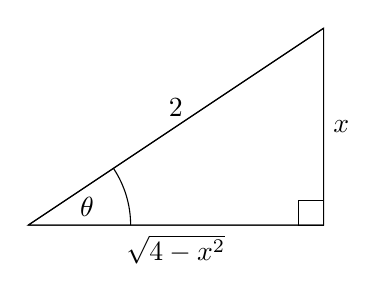
\begin{tikzpicture}[scale=1.25]
    \coordinate (A) at (-1.5cm,-1.0cm);
    \coordinate (B) at (1.5cm,1.0cm);
    \coordinate (C) at (1.5cm,-1.0cm);
    \draw (A) -- node[above]{\( 2 \)}
          (B)--node[right]{\( x \)}
          (C)--node[below]{\( \sqrt{4-x^{2}} \)}(A);
    \draw (C) -- (A) -- (B) pic [draw,angle radius=13mm,"\( \theta \)"]
          {angle=C--A--B};
    \draw (1.25cm,-1.0cm) rectangle (1.5cm,-0.75cm);
  \end{tikzpicture}
\end{center}
Therefore: \( \cot(\theta) = \frac{adj}{opp} = \frac{\sqrt{4-x^{2}}}{x} \)
\[ \frac{1}{4}\cot(\theta)+C = \frac{1}{4}\frac{\sqrt{4-x^{2}}}{x}+C \]
\[ = \frac{\sqrt{4-x^{2}}}{4x}+C \]

\subsection*{Practice Problem 4}
\[ \int{\frac{x^{2}}{\sqrt{9-x^{2}}}\diff{x}} \]
\[ Let: x = 3\sin(\theta) \]
\[ \diff{x} = 3\cos(\theta)\diff{\theta} \]
\[ \int{\frac{(3\sin(\theta))^{2}}
   {\sqrt{9-(3\sin(\theta))^{2}}}3\cos(\theta)\diff{\theta}} \]
\[ \int{\frac{27\sin^{2}(\theta)\cos(\theta)}
   {\sqrt{9-9\sin^{2}(\theta)}}\diff{\theta}} \]
\[ \int{\frac{27\sin^{2}(\theta)\cos(\theta)}
   {\sqrt{9}\sqrt{1-1\sin^{2}(\theta)}}\diff{\theta}} \]
\[ 9\int{\frac{\sin^{2}(\theta)\cos(\theta)}
   {\sqrt{cos^{2}(\theta)}}\diff{\theta}} \]
\[ 9\int{\frac{\sin^{2}(\theta)\cos(\theta)}{cos(\theta)}\diff{\theta}} \]
\[ 9\int{\sin^{2}(\theta)\diff{\theta}} \]
Using the double angle formulas:
\[ 9\int{\bigg[\frac{1}{2}-\frac{1}{2}\cos(2\theta)\bigg]\diff{\theta}} \]
\[ \frac{9}{2}\int{1-\cos(2\theta)\diff{\theta}} \]
\[ \frac{9}{2}\bigg[\theta-\frac{\sin(2\theta)}{2}\bigg]+C \]
Using the double angle formulas again:
\[ \frac{9}{2}\bigg[\theta-\frac{2\sin(\theta)\cos(\theta)}{2}\bigg]+C \]
\[ = \frac{9}{2}\bigg[\theta-\sin(\theta)\cos(\theta)\bigg]+C \]
Recall that we substituted \( x = 3\sin(\theta) \), which we can rewrite as
\( \sin(\theta) = \frac{x}{3} = \frac{opp}{hyp} \). If we imagine a triangle in
which the opposite side is \( x \) and the hypotenuse is 3, then the adjacent
side must be \( \sqrt{9-x^{2}} \).
\begin{center}
  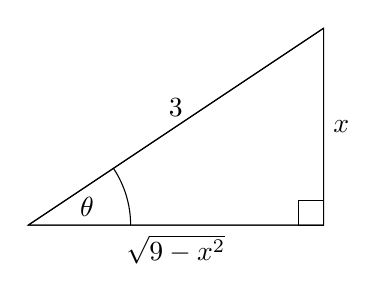
\begin{tikzpicture}[scale=1.25]
    \coordinate (A) at (-1.5cm,-1.0cm);
    \coordinate (B) at (1.5cm,1.0cm);
    \coordinate (C) at (1.5cm,-1.0cm);
    \draw (A)--node[above]{\( 3 \)}
          (B)--node[right]{\( x \)}
          (C)--node[below]{\( \sqrt{9-x^{2}} \)}(A);
    \draw (C) -- (A) -- (B) pic [draw,angle radius=13mm,"\( \theta \)"]
          {angle=C--A--B};
    \draw (1.25cm,-1.0cm) rectangle (1.5cm,-0.75cm);
  \end{tikzpicture}
\end{center}
Therefore: \( \cos(\theta) = \frac{adj}{hyp} = \frac{\sqrt{9-x^{2}}}{3} \) and
\( \theta = \arcsin(\frac{x}{3}) \)
\[ \frac{9}{2}\bigg[\theta-\sin(\theta)\cos(\theta)\bigg]+C =
   \frac{9}{2}\bigg[\arcsin(\frac{x}{3})-
   \frac{x}{3}\frac{\sqrt{9-x^{2}}}{3}\bigg]+C \]
\[ = \frac{9}{2}\bigg[\arcsin(\frac{x}{3})-
   \frac{x\sqrt{9-x^{2}}}{9}\bigg]+C \]

\subsection*{Practice Problem 6}
\[ \int_{0}^{3}{\frac{x}{\sqrt{36-x^{2}}}\diff{x}} \]
\[ Let: x = 6\sin(\theta) \]
\[ \diff{x} = 6\cos(\theta)\diff{\theta} \]
For now, we will solve the problem as an indefinite integral.
\[ \int{\frac{6\sin(\theta)}
   {\sqrt{36-(6\sin(\theta))^{2}}}6\cos(\theta)\diff{\theta}} \]
\[ \int{\frac{36\sin(\theta)\cos(\theta)}
   {\sqrt{36-36\sin^{2}(\theta)}}\diff{\theta}} \]
\[ \int{\frac{36\sin(\theta)\cos(\theta)}
   {\sqrt{36}\sqrt{1-1\sin^{2}(\theta)}}\diff{\theta}} \]
\[ 6\int{\frac{\sin(\theta)\cos(\theta)}
   {\sqrt{\cos^{2}(\theta)}}\diff{\theta}} \]
\[ 6\int{\frac{\sin(\theta)\cos(\theta)}
   {\cos(\theta)}\diff{\theta}} \]
\[ 6\int{\sin(\theta)\diff{\theta}} \]
\[ -6\cos(\theta)+C \]
Recall that we substituted \( x = 6\sin(\theta) \), which we can rewrite as
\( \sin(\theta) = \frac{x}{6} = \frac{opp}{hyp} \). If we imagine a triangle in
which the opposite side is \( x \) and the hypotenuse is 6, then the adjacent
side must be \( \sqrt{36-x^{2}} \).
\begin{center}
  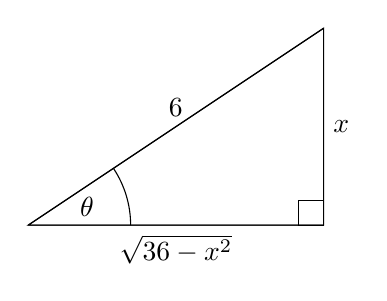
\begin{tikzpicture}[scale=1.25]
    \coordinate (A) at (-1.5cm,-1.0cm);
    \coordinate (B) at (1.5cm,1.0cm);
    \coordinate (C) at (1.5cm,-1.0cm);
    \draw (A)--node[above]{\( 6 \)}
          (B)--node[right]{\( x \)}
          (C)--node[below]{\( \sqrt{36-x^{2}} \)}(A);
    \draw (C) -- (A) -- (B) pic [draw,angle radius=13mm,"\( \theta \)"]
          {angle=C--A--B};
    \draw (1.25cm,-1.0cm) rectangle (1.5cm,-0.75cm);
  \end{tikzpicture}
\end{center}
Therefore: \( \cos(\theta) = \frac{adj}{hyp} = \frac{\sqrt{36-x^{2}}}{6} \)
\[ -6\cos(\theta)+C = -6\frac{\sqrt{36-x^{2}}}{6}+C \]
\[ = -\sqrt{36-x^{2}}+C \]
Now we can use the original limits of the intergral to solve this.
\[ \bigg[-\sqrt{36-x^{2}}\bigg]_{0}^{3} \]
\[ -\sqrt{36-3^{2}}-(-\sqrt{36-0^{2}}) \]
\[ -\sqrt{27}+6 \]
\[ = 6-3\sqrt{3} \]

\subsection*{Practice Problem 8}
\[ \int{\frac{\diff{t}}{t^{2}\sqrt{t^{2}-16}}} \]
Note that the radical is of the form \( t^{2}-16 \). We cannot subsitute
\( \sin(\theta) \) into this since it will not satisfy the trigonometric
identity.
\[ Let: x = 4\sec(\theta) \]
\[ \diff{x} = 4\sec(\theta)\tan(\theta)\diff{\theta} \]
\[ \int{\frac{4\sec{\theta}\tan(\theta)}
   {16\sec^{2}(\theta)\sqrt{(4\sec(\theta))^{2}-16}}\diff(\theta)} \]
\[ \frac{1}{4}\int{\frac{\tan(\theta)}
   {\sec(\theta)\sqrt{16}\sqrt{\sec^{2}(\theta)-1}}\diff(\theta)} \]
\[ \frac{1}{16}\int{\frac{\tan(\theta)}
   {\sec(\theta)\sqrt{\tan^{2}(\theta)}}\diff(\theta)} \]
\[ \frac{1}{16}\int{\frac{\tan(\theta)}
   {\sec(\theta)\tan(\theta)}\diff(\theta)} \]
\[ \frac{1}{16}\int{\cos(\theta)\diff{\theta}} \]
\[ \frac{1}{16}\sin(\theta)+C \]
Recall that we substituted \( x = 4\sec(\theta) \), which we can rewrite as
\( \sec(\theta) = \frac{x}{4} = \frac{hyp}{adj} \). If we imagine a triangle in
which the hypotenuse is x and the adjacent side is 4, then the opposite side
must be \( \sqrt{16-x^{2}} \).
\begin{center}
  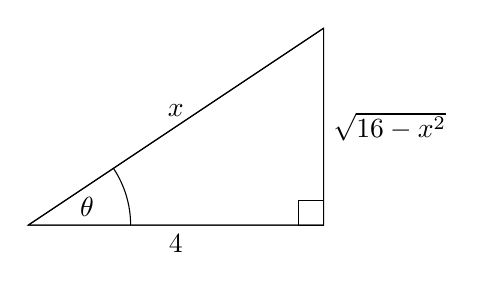
\begin{tikzpicture}[scale=1.25]
    \coordinate (A) at (-1.5cm,-1.0cm);
    \coordinate (B) at (1.5cm,1.0cm);
    \coordinate (C) at (1.5cm,-1.0cm);
    \draw (A)--node[above]{\( x \)}
          (B)--node[right]{\( \sqrt{16-x^{2}} \)}
          (C)--node[below]{\( 4 \)}(A);
    \draw (C) -- (A) -- (B) pic [draw,angle radius=13mm,"\( \theta \)"]
          {angle=C--A--B};
    \draw (1.25cm,-1.0cm) rectangle (1.5cm,-0.75cm);
  \end{tikzpicture}
\end{center}
Therefore: \( \sin(\theta) = \frac{opp}{hyp} = \frac{\sqrt{16-x^{2}}}{4} \)
\[ \frac{1}{16}\sin(\theta)+C = \frac{1}{16}\frac{\sqrt{16-x^{2}}}{4}+C \]
\[ \frac{\sqrt{16-x^{2}}}{64}+C \]

\subsection*{Practice Problem 15}
\[ \int{x^{2}\sqrt{a^{2}-x^{2}}\diff{x}} \]
\[ Let: x = a\sin(\theta)\diff{\theta} \]
\[ \diff{x} = a\cos(\theta)\diff{\theta} \]
\[ \int{a^{2}\sin^{2}(\theta)
   \sqrt{a^{2}-a^{2}\sin^{2}(\theta)}a\cos(\theta)\diff{\theta}} \]
\[ a^{4}\int{\sin^{2}(\theta)\cos(\theta)
   \sqrt{1-\sin^{2}(\theta)}\diff{\theta}} \]
\[ a^{4}\int{\sin^{2}(\theta)\cos(\theta)
   \sqrt{\cos^{2}(\theta)}\diff{\theta}} \]
\[ a^{4}\int{\sin^{2}(\theta)\cos^{2}(\theta)\diff{\theta}} \]
\[ a^{4}\int{(\sin(\theta)\cos(\theta))^{2}\diff{\theta}} \]
Using the double angle formulas:
\[ a^{4}\int{(\frac{\sin(2\theta)}{2})^{2}\diff{\theta}} \]
\[ \frac{a^{4}}{4}\int{\sin^{2}(2\theta)\diff{\theta}} \]
Using the double angle formulas again:
\[ \frac{a^{4}}{4}\int{\frac{1-\cos(4\theta)}{2}\diff{\theta}} \]
\[ \frac{a^{4}}{8}\int{1-\cos(4\theta)\diff{\theta}} \]
\[ \frac{a^{4}}{8}\bigg[\theta-\frac{1}{4}\sin(4\theta)\bigg]+C \]
\[ \frac{a^{4}}{8}\bigg[\theta-\frac{1}{4}2\sin(2\theta)\cos(2\theta)\bigg]+C \]
\[ \frac{a^{4}}{8}\bigg[\theta-
   \frac{1}{2}(2\sin(\theta)\cos(\theta))(1-2\sin^{2}(\theta))\bigg]+C \]
\[ \frac{a^{4}}{8}\bigg[\theta-
   \sin(\theta)\cos(\theta)-2\sin^{2}(\theta)\sin(\theta)\cos(\theta)\bigg]+C \]
\[ \frac{a^{4}}{8}\bigg[\theta-
   \sin(\theta)\cos(\theta)-2\sin^{3}(\theta)\cos(\theta)\bigg]+C \]
Recall that we substituted \( x = a\sin(\theta) \), which we can rewrite as
\( \sin(\theta) = \frac{x}{a} = \frac{opp}{hyp} \). If we imagine a triangle in
which the opposite side is \( x \) and the hypotenuse is \( a \), then the
adjacent side must be \( \sqrt{a^{2}-x^{2}} \).
\begin{center}
  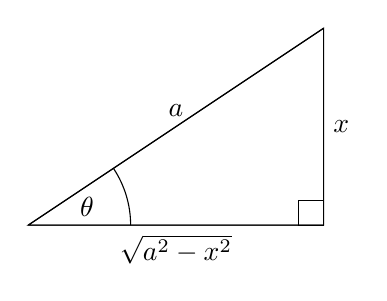
\begin{tikzpicture}[scale=1.25]
    \coordinate (A) at (-1.5cm,-1.0cm);
    \coordinate (B) at (1.5cm,1.0cm);
    \coordinate (C) at (1.5cm,-1.0cm);
    \draw (A)--node[above]{\( a \)}
          (B)--node[right]{\( x \)}
          (C)--node[below]{\( \sqrt{a^{2}-x^{2}} \)}(A);
    \draw (C) -- (A) -- (B) pic [draw,angle radius=13mm,"\( \theta \)"]
          {angle=C--A--B};
    \draw (1.25cm,-1.0cm) rectangle (1.5cm,-0.75cm);
  \end{tikzpicture}
\end{center}
Given this information:
\[ \theta = \arcsin(\frac{x}{a}) \]
\[ \sin(\theta) = \frac{x}{a} \]
\[ \cos(\theta) = \frac{\sqrt{a^{2}-x^{2}}}{a} \]
We can substitute this back into our solution:
\[ \frac{a^{4}}{8}\bigg[\theta-
\sin(\theta)\cos(\theta)-2\sin^{3}(\theta)\cos(\theta)\bigg]+C \]
\[ \frac{a^{4}}{8}\bigg[\arcsin(\frac{x}{a})-
   \frac{x\sqrt{a^{2}-x^{2}}}{a^{2}}-
   \frac{2x^{3}\sqrt{a^{2}-x^{2}}}{a^{4}}\bigg]+C \]

\subsection*{Practice Problem 21}
\[ \int{\frac{x^{2}}{\sqrt{9-25x^{2}}}\diff{x}} \]
The terms inside the radical are not of the same form as the problems
before. We can rewrite this problem to figure out the substitution.
\[ \int{\frac{x^{2}}{\sqrt{3^{2}-(5x)^{2}}}\diff{x}} \]
\[ Let: 5x = 3\sin(t) \]
\[ 5\diff{x} = 3\cos(t)\diff{t} \]
\[ \diff{x} = \frac{3}{5}\cos(t)\diff{t} \]
\[ \int{\frac{(\frac{3}{5}\sin(t))^{2}}{\sqrt{3^{2}-3^{2}\sin^{2}(t)}}
   \frac{3}{5}\cos(t)\diff{t}} \]
\[ \frac{\frac{27}{125}}{3}
   \int{\frac{\cos(t)\sin^{2}(t)}{\cos(t)}\diff{t}} \]
\[ \frac{9}{125}\int{\sin^{2}(t)\diff{t}} \]
\[ \frac{9}{125}\int{\frac{1}{2}(1-\cos(2t))\diff{t}} \]
\[ \frac{9}{250}\bigg[t-\frac{\sin(2t)}{2}\bigg]+C \]
\[ \frac{9}{250}\bigg[t-\frac{2\sin(t)\cos(t)}{2}\bigg]+C \]
\[ \frac{9}{250}\bigg[t-\sin(t)\cos(t)\bigg]+C \]
Recall that we substituted \( 5x = 3\sin(t) \), which we can rewrite as
\( \sin(t) = \frac{5x}{3} = \frac{opp}{hyp} \). If we imagine a triangle
in which the opposite side is \( 5x \) and the hypotenuse is 3, then the
adjacent side is \( \sqrt{9-25x^{2}} \).
\begin{center}
  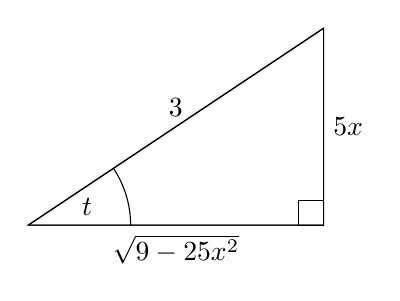
\begin{tikzpicture}[scale=1.25]
    \coordinate (A) at (-1.5cm,-1.0cm);
    \coordinate (B) at (1.5cm,1.0cm);
    \coordinate (C) at (1.5cm,-1.0cm);
    \draw (A)--node[above]{\( 3 \)}
          (B)--node[right]{\( 5x \)}
          (C)--node[below]{\( \sqrt{9-25x^{2}} \)}(A);
    \draw (C) -- (A) -- (B) pic [draw,angle radius=13mm,"\( t \)"]
          {angle=C--A--B};
    \draw (1.25cm,-1.0cm) rectangle (1.5cm,-0.75cm);
  \end{tikzpicture}
\end{center}
Therefore: \( \cos(t) = \frac{adj}{hyp} = \frac{\sqrt{9-25x^{2}}}{3} \)
and \( t = \arcsin(\frac{5x}{3}) \)
\[ \frac{9}{250}\bigg[t-\sin(t)\cos(t)\bigg]+C \]
\[ \frac{9}{250}\bigg[\arcsin(\frac{5x}{3})-
   \frac{5x}{3}\frac{\sqrt{9-25x^{2}}}{3}\bigg]+C \]
\[ \frac{9}{250}\bigg[\arcsin(\frac{5x}{3})-
   \frac{5x\sqrt{9-25x^{2}}}{9}\bigg]+C \]

\subsection*{Practice Problem 27}
\[ \int{\sqrt{x^{2}+2x}\diff{x}} \]
This problem requires a different approach. We need to turn this into the form
of a trigonometric substitution problem.
\[ \int{\sqrt{x^{2}+2x}\diff{x}} = \int{\sqrt{x^{2}+2x+(1-1)}\diff{x}} \]
\[ \int{\sqrt{x^{2}+2x+1-1}\diff{x}} \]
\[ \int{\sqrt{(x+1)^{2}-1}\diff{x}} \]
\[ Let: x+1 = \sec(\theta) \]
\[ \diff{x} = \sec(\theta)\tan(\theta)\diff{\theta} \]
\[ \int{\sqrt{\sec^{2}(\theta)-1}\sec(\theta)\tan(\theta)\diff{\theta}} \]
\[ \int{\sqrt{\tan^{2}(\theta)}\sec(\theta)\tan(\theta)\diff{\theta}} \]
\[ \int{\tan^{2}(\theta)\sec(\theta)\diff{\theta}} \]
Now we use integration by parts:
\[ Let: f(x) = \tan(\theta) \quad
   g'(x) = \tan(\theta)\sec(\theta)\diff{\theta} \]
\[ f'(x) = \sec^{2}(\theta)\diff{\theta} \quad g(x) = \sec(\theta) \]
\[ \int{\tan^{2}(\theta)\sec(\theta)\diff{\theta}} =
   \tan(\theta)\sec(\theta)-\int{\sec^{2}(\theta)\sec(\theta)\diff{\theta}} \]
\[ \int{\tan^{2}(\theta)\sec(\theta)\diff{\theta}} =
   \tan(\theta)\sec(\theta)-
   \int{(\tan^{2}(\theta)+1)\sec(\theta)\diff{\theta}} \]
\[ \int{\tan^{2}(\theta)\sec(\theta)\diff{\theta}} =
   \tan(\theta)\sec(\theta)-\int{\tan^{2}(\theta)\sec(\theta)\diff(\theta)}+
   \int{\sec(\theta)\diff{\theta}} \]
\[ 2\int{\tan^{2}(\theta)\sec(\theta)\diff{\theta}} =
   \tan(\theta)\sec(\theta)-\int{\sec(\theta)\diff{\theta}} \]
\[ 2\int{\tan^{2}(\theta)\sec(\theta)\diff{\theta}} =
   \tan(\theta)\sec(\theta)-\ln|\sec(x)+\tan(x)|+C \]
\[ \int{\tan^{2}(\theta)\sec(\theta)\diff{\theta}} =
   \frac{1}{2}\tan(\theta)\sec(\theta)-\frac{1}{2}\ln|\sec(x)+\tan(x)|+C \]
Recall that we substituted \( x+1 = \sec(\theta) \), which we can rewrite as
\( \sec(\theta) = \frac{x+1}{1} = \frac{hyp}{adj} \). If we imagine a triangle
in which the hypotenuse is \( x+1 \) and the adjacent side is 1, then the
opposite side must be \( \sqrt{x} \).
\begin{center}
  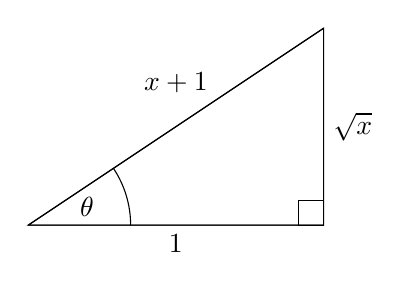
\begin{tikzpicture}[scale=1.25]
    \coordinate (A) at (-1.5cm,-1.0cm);
    \coordinate (B) at (1.5cm,1.0cm);
    \coordinate (C) at (1.5cm,-1.0cm);
    \draw (A)--node[above=0.3cm]{\( x+1 \)}
          (B)--node[right]{\( \sqrt{x} \)}
          (C)--node[below]{\( 1 \)}(A);
    \draw (C) -- (A) -- (B) pic [draw,angle radius=13mm,"\( \theta \)"]
          {angle=C--A--B};
    \draw (1.25cm,-1.0cm) rectangle (1.5cm,-0.75cm);
  \end{tikzpicture}
\end{center}
Therefore: \( \tan(\theta) = \frac{opp}{adj} = \frac{\sqrt{x}}{1} \)
\[ \frac{1}{2}\tan(\theta)\sec(\theta)-\frac{1}{2}\ln|\sec(x)+\tan(x)|+C =
   \frac{1}{2}\sqrt{x}(x+1)-\frac{1}{2}\ln|(x+1)+\sqrt{x}|+C \]
\[ = \frac{\sqrt{x}(x+1)}{2}-\frac{\ln|x+\sqrt{x}+1|}{2}+C \]

\subsection*{Practice Problem 45}
\[ \int{x^{3}\sqrt{1+x^{2}}\diff{x}} \]
For this problem, we can solve it with regular substitution:
\[ \int{x^{2}x\sqrt{1+x^{2}}\diff{x}} \]
\[ Let: 1+x^{2} = t \]
\[ x\diff{x} = \frac{\diff{t}}{2} \]
\[ \frac{1}{2}\int{(t-1)t^{\frac{1}{2}}\diff{t}} \]
\[ \frac{1}{2}\int{t^{\frac{3}{2}}-t^{\frac{1}{2}}\diff{t}} \]
\[ = \frac{1}{2}\bigg[\frac{t^{\frac{5}{2}}}{\frac{5}{2}}-
     \frac{t^{\frac{3}{2}}}{\frac{2}{2}}+C\bigg] \]
But we can also use trigonometric substitution:
\[ \int{x^{3}\sqrt{1+x^{2}}\diff{x}} \]
\[ Let: x = \tan(\theta) \]
\[ \diff{x} = \sec^{2}(\theta)\diff{\theta} \]
\[ \int{\tan^{3}(\theta)\sqrt{1+\tan^{2}(\theta)}
   \sec^{2}(\theta)\diff{\theta}} \]
\[ \int{\tan^{3}(\theta)\sqrt{\sec^{2}(\theta)}
   \sec^{2}(\theta)\diff{\theta}} \]
\[ \int{\tan^{3}(\theta)\sec^{3}(\theta)\diff{\theta}} \]
\[ \int{\tan(\theta)\tan^{2}(\theta)\sec^{3}(\theta)\diff{\theta}} \]
\[ \int{\tan(\theta)(\sec^{2}-1)\sec^{3}(\theta)\diff{\theta}} \]
\[ \int{\tan(\theta)\sec^{5}(\theta)\diff{\theta}}-
   \int{\tan(\theta)\sec^{3}(\theta)\diff{\theta}} \]
\[ \int{\tan(\theta)\sec(\theta)\sec^{4}(\theta)\diff{\theta}}-
   \int{\tan(\theta)\sec(\theta)\sec^{2}(\theta)\diff{\theta}} \]
\[ Let: u = \sec(\theta) \]
\[ \diff{u} = \sec(\theta)\tan(\theta)\diff{\theta} \]
\[ \int{u^{4}\diff{u}}- \int{u^{2}\diff{u}} \]
\[ \frac{u^{5}}{5}-\frac{u^{3}}{3}+C \]
\[ \frac{\sec^{5}(\theta)}{5}-\frac{\sec^{3}(\theta)}{3}+C \]
Recall that we substituted \( x = \tan(\theta) \), which we can rewrite as
\( \tan(\theta) = \frac{x}{1} = \frac{opp}{adj} \). If we imagine a triangle in
which the opposite side is \( x \) and the adjacent side is 1, then the
hypotenuse must be \( \sqrt{1+x^{2}} \).
\begin{center}
  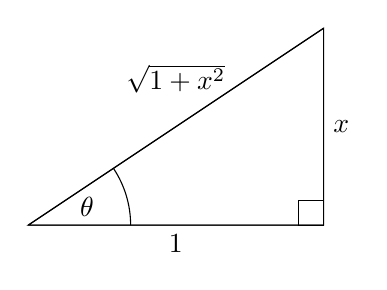
\begin{tikzpicture}[scale=1.25]
    \coordinate (A) at (-1.5cm,-1.0cm);
    \coordinate (B) at (1.5cm,1.0cm);
    \coordinate (C) at (1.5cm,-1.0cm);
    \draw (A)--node[above=0.3cm]{\( \sqrt{1+x^{2}} \)}
          (B)--node[right]{\( x \)}
          (C)--node[below]{\( 1 \)}(A);
    \draw (C) -- (A) -- (B) pic [draw,angle radius=13mm,"\( \theta \)"]
          {angle=C--A--B};
    \draw (1.25cm,-1.0cm) rectangle (1.5cm,-0.75cm);
  \end{tikzpicture}
\end{center}
Therefore: \( sec(\theta) = \frac{hyp}{adj} = \frac{\sqrt{1+x^{2}}}{1} \).
\[ \frac{\sec^{5}(\theta)}{5}-\frac{\sec^{3}(\theta)}{3}+C =
   \frac{1}{5}(\sqrt{1+x^{2}})^{5}-\frac{1}{3}(\sqrt{1+x^{2}})^{3}+C \]
\[ = \frac{(1+x^{2})^{\frac{5}{2}}}{5}-\frac{(1+x^{2})^{\frac{3}{2}}}{3}+C \]

\subsection*{Follow-up Questions}
\[ \int{x^{2}\sqrt{3-2x-x^{2}}\diff{x}} \]
\[ \int{x^{2}\sqrt{-(x^{2}+2x-3)}\diff{x}} \]
\[ \int{x^{2}\sqrt{-(x^{2}+2x-3+4-4)}\diff{x}} \]
\[ \int{x^{2}\sqrt{-(x^{2}+2x+1)+4}\diff{x}} \]
\[ \int{x^{2}\sqrt{4-(x+1)^{2}}\diff{x}} \]
\[ Let: x + 1 = 2\cos(\theta) \]
\[ \diff{x} = -2\sin(\theta)\diff{\theta} \]
\[ \int{(2\cos(\theta)-1)^{2}\sqrt{4-(2\cos(\theta))^{2}}
   (-2\sin(\theta))\diff{\theta}} \]
\[ -2\int{(2\cos(\theta)-1)^{2}\sqrt{4}\sqrt{1-cos^{2}(\theta)}
   (-2\sin(\theta))\diff{\theta}} \]
\[ -4\int{(2\cos(\theta)-1)^{2}\sqrt{\sin^{2}(\theta)}
   (-\sin(\theta))\diff{\theta}} \]
\[ -4\int{(4\cos^{2}(\theta)-4\cos(\theta)+1)
   (-\sin^{2}(\theta))\diff{\theta}} \]
\[ 4\int{4\cos^{2}(\theta)\sin^{2}(\theta)-4\cos(\theta)\sin^{2}(\theta)+
   \sin^{2}(\theta)\diff{\theta}} \]
\[ 16\int{\cos^{2}(\theta)\sin^{2}(\theta)\diff{\theta}}-
   16\int{\cos(\theta)\sin^{2}(\theta)\diff{\theta}}-
   4\int{\sin^{2}(\theta)\diff{\theta}} \]
\[ 4\int{(2\cos^{2}(\theta)\sin^{2}(\theta))^{2}\diff{\theta}}-
   16\int{\cos(\theta)\sin^{2}(\theta)\diff{\theta}}-
   2\int{2\sin^{2}(\theta)\diff{\theta}} \]
\[ 4\int{\sin^{2}(2\theta)\diff{\theta}}-
   16\int{\cos(\theta)\sin^{2}(\theta)\diff{\theta}}-
   2\int{1-\cos(2\theta)\diff{\theta}} \]
\[ \bigg[2\int{2\sin^{2}(2\theta)\diff{\theta}}\bigg]-
   \bigg[16\frac{\cos^{3}(\theta)}{3}\bigg]-
   \bigg[(2\theta-\sin(2\theta))\bigg]+C \]
\[ \bigg[\int{1-\cos(4\theta)\diff{\theta}}\bigg]-
   \bigg[16\frac{\cos^{3}(\theta)}{3}\bigg]-
   \bigg[(2\theta-\sin(2\theta))\bigg]+C \]
\[ \bigg[2\theta-\frac{\sin(4\theta)}{2}\bigg]-
   \bigg[16\frac{\cos^{3}(\theta)}{3}\bigg]-
   \bigg[(2\theta-\sin(2\theta))\bigg]+C \]
\[ 2\theta-\frac{\sin(4\theta)}{2}-
   \frac{16\cos^{3}(\theta)}{3}-
   2\theta+\sin(2\theta)+C \]
\[ \sin(2\theta)-\frac{\sin(4\theta)}{2}-\frac{16\cos^{3}(\theta)}{3}+C \]
\[ 2\sin(\theta)\cos(\theta)-
   \frac{2\sin(2\theta)\cos(2\theta)}{2}-
   \frac{16\cos^{3}(\theta)}{3}+C \]
\[ 2\sin(\theta)\cos(\theta)-
   \frac{2(2\sin(\theta)\cos(\theta))(2\cos^{2}(\theta)-1)}{2}-
   \frac{16\cos^{3}(\theta)}{3}+C \]
\[ 2\sin(\theta)\cos(\theta)-
   (2\sin(\theta)\cos(\theta))(2\cos^{2}(\theta)-1)-
   \frac{16\cos^{3}(\theta)}{3}+C \]
Recall that we substituted \( x+1 = 2\cos(\theta) \), which we can rewrite as
\(\cos(\theta) = \frac{x+1}{2} = \frac{adj}{hyp} \). If we imagine a triangle
in which the adjacent side is \( x+1 \) and the hypotenuse is 2, then the
opposide side must be \( \sqrt{4-(x+1)^{2}} \), or \( \sqrt{2-2x-x^{2}} \).
\begin{center}
  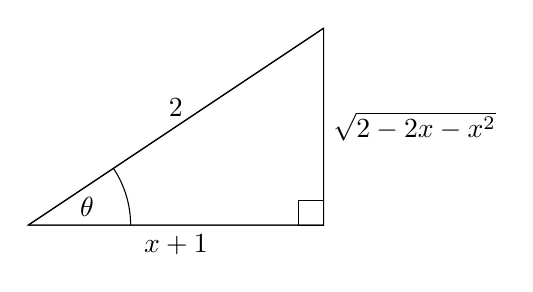
\begin{tikzpicture}[scale=1.25]
    \coordinate (A) at (-1.5cm,-1.0cm);
    \coordinate (B) at (1.5cm,1.0cm);
    \coordinate (C) at (1.5cm,-1.0cm);
    \draw (A)--node[above]{\( 2 \)}
          (B)--node[right]{\( \sqrt{2-2x-x^{2}} \)}
          (C)--node[below]{\( x+1 \)}(A);
    \draw (C) -- (A) -- (B) pic [draw,angle radius=13mm,"\( \theta \)"]
          {angle=C--A--B};
    \draw (1.25cm,-1.0cm) rectangle (1.5cm,-0.75cm);
  \end{tikzpicture}
\end{center}
Therefore: \( \sin(\theta) = \frac{\sqrt{2-2x-x^{2}}}{2} \)
\[ 2\sin(\theta)\cos(\theta)-
   (2\sin(\theta)\cos(\theta))(2\cos^{2}(\theta)-1)-
   \frac{16\cos^{3}(\theta)}{3}+C \]
\[ 2\frac{\sqrt{2-2x-x^{2}}}{2}\frac{x+1}{2}-
   (2\frac{\sqrt{2-2x-x^{2}}}{2}\frac{x+1}{2})(2(\frac{x+1}{2})^{2}-1)-
   \frac{16(\frac{x+1}{2})^{3}}{3}+C \]
\[ \frac{(x+1)\sqrt{2-2x-x^{2}}}{2}-
   \frac{(x+1)\sqrt{2-2x-x^{2}}}{2}(\frac{(x+1)^{2}}{2}-1)-
   \frac{16}{3}(\frac{x+1}{2})^{3}+C \]
\[ = \frac{-(x+1)^{3}\sqrt{2-2x-x^{2}}}{2}-\frac{2(x+1)^{3}}{3}+C \]

\begin{center}
  If any errors are found, please contact me at alvin.lin.dev@gmail.com
\end{center}

\end{document}
